\documentclass[1p]{elsarticle_modified}
%\bibliographystyle{elsarticle-num}

%\usepackage[colorlinks]{hyperref}
%\usepackage{abbrmath_seonhwa} %\Abb, \Ascr, \Acal ,\Abf, \Afrak
\usepackage{amsfonts}
\usepackage{amssymb}
\usepackage{amsmath}
\usepackage{amsthm}
\usepackage{scalefnt}
\usepackage{amsbsy}
\usepackage{kotex}
\usepackage{caption}
\usepackage{subfig}
\usepackage{color}
\usepackage{graphicx}
\usepackage{xcolor} %% white, black, red, green, blue, cyan, magenta, yellow
\usepackage{float}
\usepackage{setspace}
\usepackage{hyperref}

\usepackage{tikz}
\usetikzlibrary{arrows}

\usepackage{multirow}
\usepackage{array} % fixed length table
\usepackage{hhline}

%%%%%%%%%%%%%%%%%%%%%
\makeatletter
\renewcommand*\env@matrix[1][\arraystretch]{%
	\edef\arraystretch{#1}%
	\hskip -\arraycolsep
	\let\@ifnextchar\new@ifnextchar
	\array{*\c@MaxMatrixCols c}}
\makeatother %https://tex.stackexchange.com/questions/14071/how-can-i-increase-the-line-spacing-in-a-matrix
%%%%%%%%%%%%%%%

\usepackage[normalem]{ulem}

\newcommand{\msout}[1]{\ifmmode\text{\sout{\ensuremath{#1}}}\else\sout{#1}\fi}
%SOURCE: \msout is \stkout macro in https://tex.stackexchange.com/questions/20609/strikeout-in-math-mode

\newcommand{\cancel}[1]{
	\ifmmode
	{\color{red}\msout{#1}}
	\else
	{\color{red}\sout{#1}}
	\fi
}

\newcommand{\add}[1]{
	{\color{blue}\uwave{#1}}
}

\newcommand{\replace}[2]{
	\ifmmode
	{\color{red}\msout{#1}}{\color{blue}\uwave{#2}}
	\else
	{\color{red}\sout{#1}}{\color{blue}\uwave{#2}}
	\fi
}

\newcommand{\Sol}{\mathcal{S}} %segment
\newcommand{\D}{D} %diagram
\newcommand{\A}{\mathcal{A}} %arc


%%%%%%%%%%%%%%%%%%%%%%%%%%%%%5 test

\def\sl{\operatorname{\textup{SL}}(2,\Cbb)}
\def\psl{\operatorname{\textup{PSL}}(2,\Cbb)}
\def\quan{\mkern 1mu \triangleright \mkern 1mu}

\theoremstyle{definition}
\newtheorem{thm}{Theorem}[section]
\newtheorem{prop}[thm]{Proposition}
\newtheorem{lem}[thm]{Lemma}
\newtheorem{ques}[thm]{Question}
\newtheorem{cor}[thm]{Corollary}
\newtheorem{defn}[thm]{Definition}
\newtheorem{exam}[thm]{Example}
\newtheorem{rmk}[thm]{Remark}
\newtheorem{alg}[thm]{Algorithm}

\newcommand{\I}{\sqrt{-1}}
\begin{document}

%\begin{frontmatter}
%
%\title{Boundary parabolic representations of knots up to 8 crossings}
%
%%% Group authors per affiliation:
%\author{Yunhi Cho} 
%\address{Department of Mathematics, University of Seoul, Seoul, Korea}
%\ead{yhcho@uos.ac.kr}
%
%
%\author{Seonhwa Kim} %\fnref{s_kim}}
%\address{Center for Geometry and Physics, Institute for Basic Science, Pohang, 37673, Korea}
%\ead{ryeona17@ibs.re.kr}
%
%\author{Hyuk Kim}
%\address{Department of Mathematical Sciences, Seoul National University, Seoul 08826, Korea}
%\ead{hyukkim@snu.ac.kr}
%
%\author{Seokbeom Yoon}
%\address{Department of Mathematical Sciences, Seoul National University, Seoul, 08826,  Korea}
%\ead{sbyoon15@snu.ac.kr}
%
%\begin{abstract}
%We find all boundary parabolic representation of knots up to 8 crossings.
%
%\end{abstract}
%\begin{keyword}
%    \MSC[2010] 57M25 
%\end{keyword}
%
%\end{frontmatter}

%\linenumbers
%\tableofcontents
%
\newcommand\colored[1]{\textcolor{white}{\rule[-0.35ex]{0.8em}{1.4ex}}\kern-0.8em\color{red} #1}%
%\newcommand\colored[1]{\textcolor{white}{ #1}\kern-2.17ex	\textcolor{white}{ #1}\kern-1.81ex	\textcolor{white}{ #1}\kern-2.15ex\color{red}#1	}

{\Large $\underline{12a_{0079}~(K12a_{0079})}$}

\setlength{\tabcolsep}{10pt}
\renewcommand{\arraystretch}{1.6}
\vspace{1cm}\begin{tabular}{m{100pt}>{\centering\arraybackslash}m{274pt}}
\multirow{5}{120pt}{
	\centering
	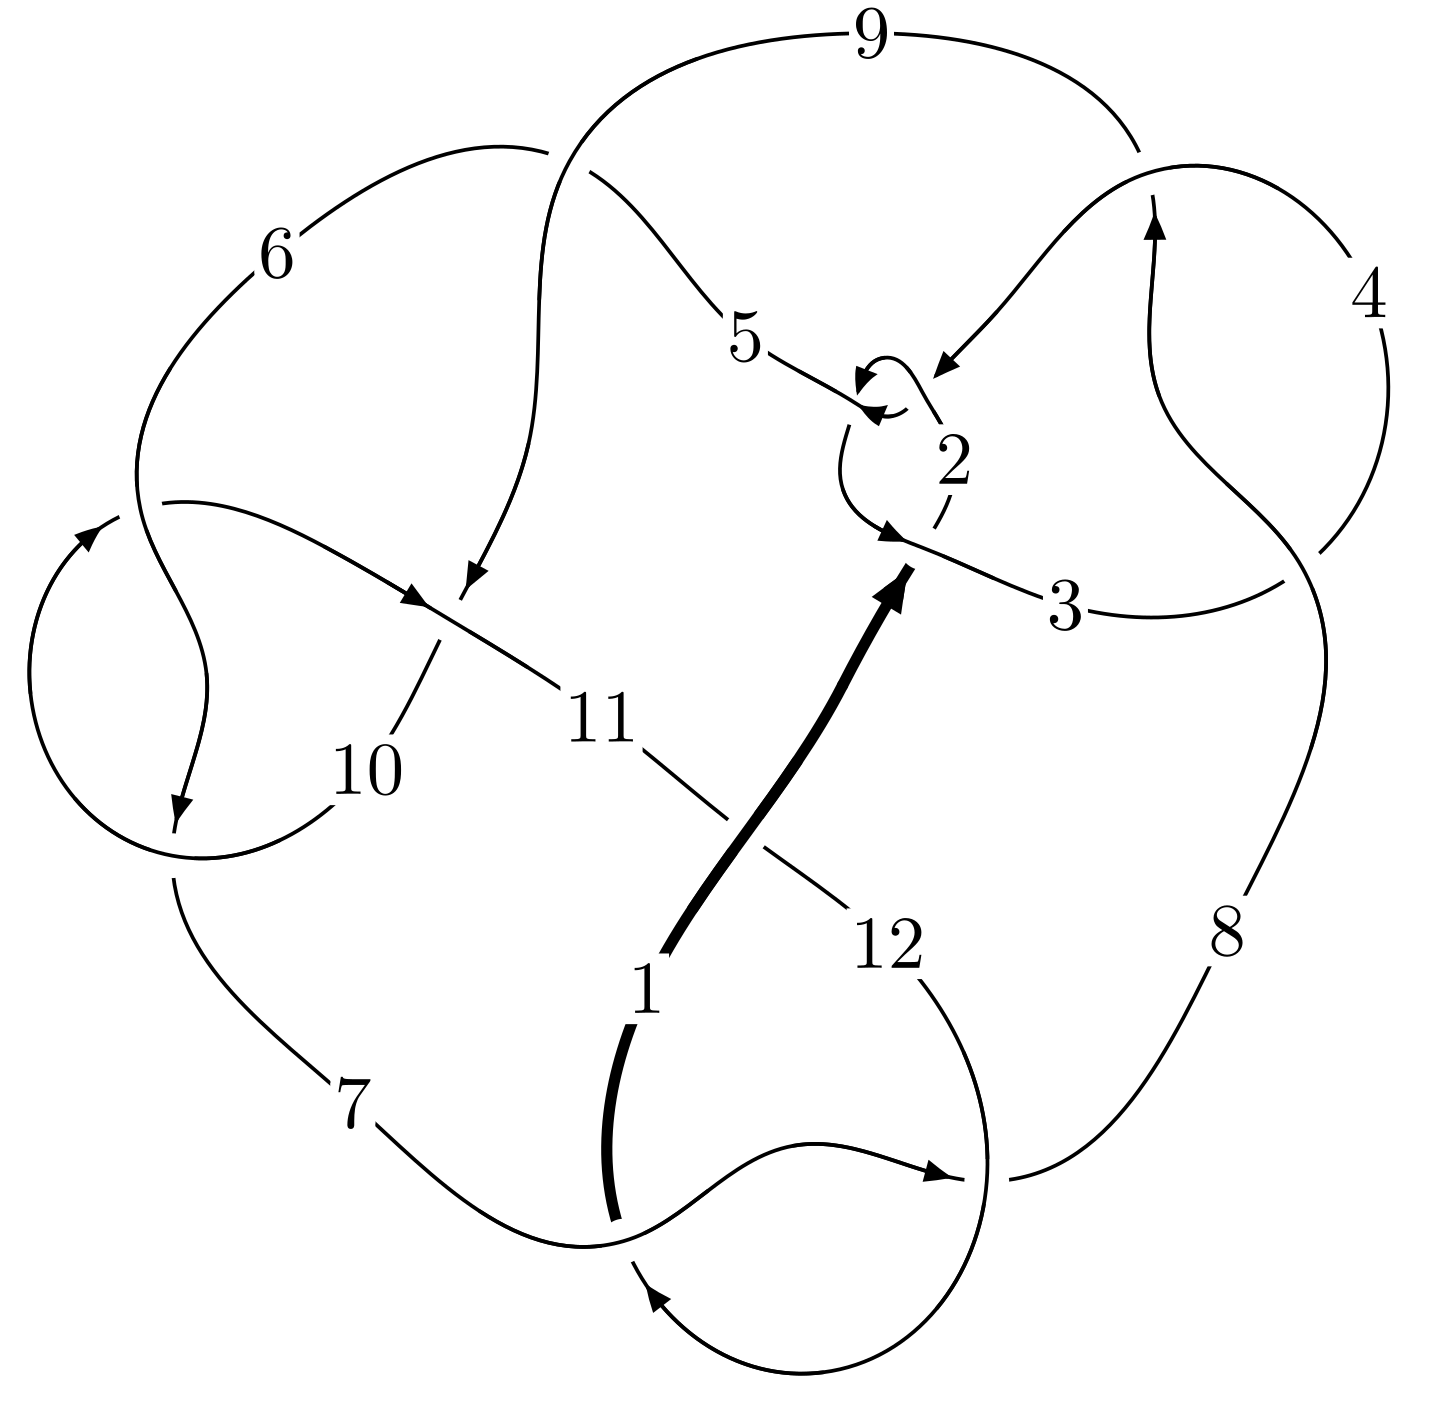
\includegraphics[width=112pt]{../../../GIT/diagram.site/Diagrams/png/880_12a_0079.png}\\
\ \ \ A knot diagram\footnotemark}&
\allowdisplaybreaks
\textbf{Linearized knot diagam} \\
\cline{2-2}
 &
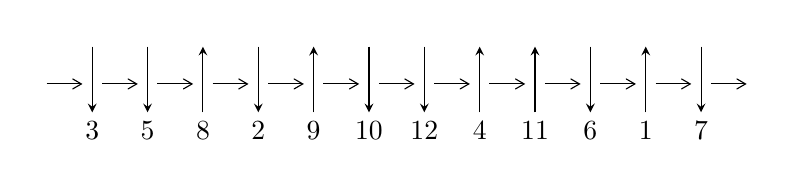
\begin{tikzpicture}[x=20pt, y=17pt]
	% nodes
	\node (C0) at (0, 0) {};
	\node (C1) at (1, 0) {};
	\node (C1U) at (1, +1) {};
	\node (C1D) at (1, -1) {3};

	\node (C2) at (2, 0) {};
	\node (C2U) at (2, +1) {};
	\node (C2D) at (2, -1) {5};

	\node (C3) at (3, 0) {};
	\node (C3U) at (3, +1) {};
	\node (C3D) at (3, -1) {8};

	\node (C4) at (4, 0) {};
	\node (C4U) at (4, +1) {};
	\node (C4D) at (4, -1) {2};

	\node (C5) at (5, 0) {};
	\node (C5U) at (5, +1) {};
	\node (C5D) at (5, -1) {9};

	\node (C6) at (6, 0) {};
	\node (C6U) at (6, +1) {};
	\node (C6D) at (6, -1) {10};

	\node (C7) at (7, 0) {};
	\node (C7U) at (7, +1) {};
	\node (C7D) at (7, -1) {12};

	\node (C8) at (8, 0) {};
	\node (C8U) at (8, +1) {};
	\node (C8D) at (8, -1) {4};

	\node (C9) at (9, 0) {};
	\node (C9U) at (9, +1) {};
	\node (C9D) at (9, -1) {11};

	\node (C10) at (10, 0) {};
	\node (C10U) at (10, +1) {};
	\node (C10D) at (10, -1) {6};

	\node (C11) at (11, 0) {};
	\node (C11U) at (11, +1) {};
	\node (C11D) at (11, -1) {1};

	\node (C12) at (12, 0) {};
	\node (C12U) at (12, +1) {};
	\node (C12D) at (12, -1) {7};
	\node (C13) at (13, 0) {};

	% arrows
	\draw[->,>={angle 60}]
	(C0) edge (C1) (C1) edge (C2) (C2) edge (C3) (C3) edge (C4) (C4) edge (C5) (C5) edge (C6) (C6) edge (C7) (C7) edge (C8) (C8) edge (C9) (C9) edge (C10) (C10) edge (C11) (C11) edge (C12) (C12) edge (C13) ;	\draw[->,>=stealth]
	(C1U) edge (C1D) (C2U) edge (C2D) (C3D) edge (C3U) (C4U) edge (C4D) (C5D) edge (C5U) (C6U) edge (C6D) (C7U) edge (C7D) (C8D) edge (C8U) (C9D) edge (C9U) (C10U) edge (C10D) (C11D) edge (C11U) (C12U) edge (C12D) ;
	\end{tikzpicture} \\
\hhline{~~} \\& 
\textbf{Solving Sequence} \\ \cline{2-2} 
 &
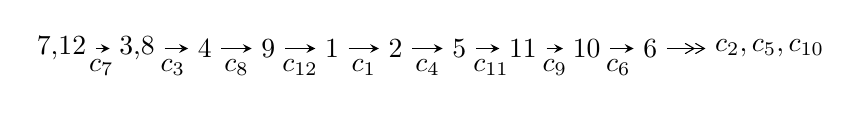
\begin{tikzpicture}[x=23pt, y=7pt]
	% node
	\node (A0) at (-1/8, 0) {7,12};
	\node (A1) at (17/16, 0) {3,8};
	\node (A2) at (17/8, 0) {4};
	\node (A3) at (25/8, 0) {9};
	\node (A4) at (33/8, 0) {1};
	\node (A5) at (41/8, 0) {2};
	\node (A6) at (49/8, 0) {5};
	\node (A7) at (57/8, 0) {11};
	\node (A8) at (65/8, 0) {10};
	\node (A9) at (73/8, 0) {6};
	\node (C1) at (1/2, -1) {$c_{7}$};
	\node (C2) at (13/8, -1) {$c_{3}$};
	\node (C3) at (21/8, -1) {$c_{8}$};
	\node (C4) at (29/8, -1) {$c_{12}$};
	\node (C5) at (37/8, -1) {$c_{1}$};
	\node (C6) at (45/8, -1) {$c_{4}$};
	\node (C7) at (53/8, -1) {$c_{11}$};
	\node (C8) at (61/8, -1) {$c_{9}$};
	\node (C9) at (69/8, -1) {$c_{6}$};
	\node (A10) at (11, 0) {$c_{2},c_{5},c_{10}$};

	% edge
	\draw[->,>=stealth]	
	(A0) edge (A1) (A1) edge (A2) (A2) edge (A3) (A3) edge (A4) (A4) edge (A5) (A5) edge (A6) (A6) edge (A7) (A7) edge (A8) (A8) edge (A9) ;
	\draw[->>,>={angle 60}]	
	(A9) edge (A10);
\end{tikzpicture} \\ 

\end{tabular} \\

\footnotetext{
The image of knot diagram is generated by the software ``\textbf{Draw programme}" developed by Andrew Bartholomew(\url{http://www.layer8.co.uk/maths/draw/index.htm\#Running-draw}), where we modified some parts for our purpose(\url{https://github.com/CATsTAILs/LinksPainter}).
}\phantom \\ \newline 
\centering \textbf{Ideals for irreducible components\footnotemark of $X_{\text{par}}$} 
 
\begin{align*}
I^u_{1}&=\langle 
-37 u^{43}-23 u^{42}+\cdots+64 b+15,\;-81 u^{43}-51 u^{42}+\cdots+64 a-37,\;u^{44}+11 u^{42}+\cdots- u+1\rangle \\
I^u_{2}&=\langle 
7.20931\times10^{43} u^{71}+8.12549\times10^{43} u^{70}+\cdots+4.80383\times10^{43} b+1.14427\times10^{45},\\
\phantom{I^u_{2}}&\phantom{= \langle  }3.81637\times10^{44} u^{71}+4.59955\times10^{44} u^{70}+\cdots+8.16652\times10^{44} a+1.32091\times10^{46},\;u^{72}+2 u^{71}+\cdots+36 u+17\rangle \\
I^u_{3}&=\langle 
- u^3+u^2+2 b+1,\;- u^3- u^2+2 a-2 u+1,\;u^4+u^2- u+1\rangle \\
I^u_{4}&=\langle 
- a^2-2 a u+2 b-2 u,\;a^3+2 a^2 u+2 a^2+2 a u+2 u-2,\;u^2+1\rangle \\
I^u_{5}&=\langle 
- u^4- u^3- u^2+b- u-1,\;- u^5- u^3- u^2+a- u-1,\;u^6+u^5+2 u^4+2 u^3+2 u^2+2 u+1\rangle \\
\\
\end{align*}
\raggedright * 5 irreducible components of $\dim_{\mathbb{C}}=0$, with total 132 representations.\\
\footnotetext{All coefficients of polynomials are rational numbers. But the coefficients are sometimes approximated in decimal forms when there is not enough margin.}
\newpage
\renewcommand{\arraystretch}{1}
\centering \section*{I. $I^u_{1}= \langle -37 u^{43}-23 u^{42}+\cdots+64 b+15,\;-81 u^{43}-51 u^{42}+\cdots+64 a-37,\;u^{44}+11 u^{42}+\cdots- u+1 \rangle$}
\flushleft \textbf{(i) Arc colorings}\\
\begin{tabular}{m{7pt} m{180pt} m{7pt} m{180pt} }
\flushright $a_{7}=$&$\begin{pmatrix}1\\0\end{pmatrix}$ \\
\flushright $a_{12}=$&$\begin{pmatrix}0\\u\end{pmatrix}$ \\
\flushright $a_{3}=$&$\begin{pmatrix}1.26563 u^{43}+0.796875 u^{42}+\cdots-0.218750 u+0.578125\\0.578125 u^{43}+0.359375 u^{42}+\cdots+1.28125 u-0.234375\end{pmatrix}$ \\
\flushright $a_{8}=$&$\begin{pmatrix}1\\u^2\end{pmatrix}$ \\
\flushright $a_{4}=$&$\begin{pmatrix}2.45313 u^{43}+1.48438 u^{42}+\cdots+1.53125 u+1.14063\\0.765625 u^{43}-0.203125 u^{42}+\cdots+0.781250 u-0.921875\end{pmatrix}$ \\
\flushright $a_{9}=$&$\begin{pmatrix}-\frac{1}{8} u^{42}-\frac{5}{4} u^{40}+\cdots-\frac{7}{8} u-\frac{1}{8}\\- u^5- u^3- u\end{pmatrix}$ \\
\flushright $a_{1}=$&$\begin{pmatrix}- u\\u\end{pmatrix}$ \\
\flushright $a_{2}=$&$\begin{pmatrix}-0.140625 u^{43}-0.0468750 u^{42}+\cdots-2.15625 u-0.578125\\-0.140625 u^{43}+0.328125 u^{42}+\cdots-0.0312500 u+0.0468750\end{pmatrix}$ \\
\flushright $a_{5}=$&$\begin{pmatrix}-\frac{1}{8} u^{43}-\frac{5}{4} u^{41}+\cdots-\frac{1}{8} u+1\\u^8+2 u^6+2 u^4\end{pmatrix}$ \\
\flushright $a_{11}=$&$\begin{pmatrix}- u^3\\u^3+u\end{pmatrix}$ \\
\flushright $a_{10}=$&$\begin{pmatrix}-\frac{1}{8} u^{42}-\frac{5}{4} u^{40}+\cdots-\frac{7}{8} u-\frac{1}{8}\\- u\end{pmatrix}$ \\
\flushright $a_{6}=$&$\begin{pmatrix}-\frac{1}{8} u^{43}-\frac{5}{4} u^{41}+\cdots-\frac{1}{8} u+1\\- u^2\end{pmatrix}$\\&\end{tabular}
\flushleft \textbf{(ii) Obstruction class $= -1$}\\~\\
\flushleft \textbf{(iii) Cusp Shapes $= -\frac{237}{128} u^{43}+\frac{161}{128} u^{42}+\cdots-\frac{897}{64} u+\frac{503}{128}$}\\~\\
\newpage\renewcommand{\arraystretch}{1}
\flushleft \textbf{(iv) u-Polynomials at the component}\newline \\
\begin{tabular}{m{50pt}|m{274pt}}
Crossings & \hspace{64pt}u-Polynomials at each crossing \\
\hline $$\begin{aligned}c_{1}\end{aligned}$$&$\begin{aligned}
&u^{44}+19 u^{43}+\cdots+97 u+16
\end{aligned}$\\
\hline $$\begin{aligned}c_{2},c_{4}\end{aligned}$$&$\begin{aligned}
&u^{44}-5 u^{43}+\cdots-5 u+4
\end{aligned}$\\
\hline $$\begin{aligned}c_{3},c_{8}\end{aligned}$$&$\begin{aligned}
&u^{44}+3 u^{43}+\cdots+368 u+64
\end{aligned}$\\
\hline $$\begin{aligned}c_{5}\end{aligned}$$&$\begin{aligned}
&u^{44}-6 u^{43}+\cdots+256 u+256
\end{aligned}$\\
\hline $$\begin{aligned}c_{6},c_{7},c_{10}\\c_{12}\end{aligned}$$&$\begin{aligned}
&u^{44}+11 u^{42}+\cdots- u+1
\end{aligned}$\\
\hline $$\begin{aligned}c_{9},c_{11}\end{aligned}$$&$\begin{aligned}
&u^{44}-22 u^{43}+\cdots-5 u+1
\end{aligned}$\\
\hline
\end{tabular}\\~\\
\newpage\renewcommand{\arraystretch}{1}
\flushleft \textbf{(v) Riley Polynomials at the component}\newline \\
\begin{tabular}{m{50pt}|m{274pt}}
Crossings & \hspace{64pt}Riley Polynomials at each crossing \\
\hline $$\begin{aligned}c_{1}\end{aligned}$$&$\begin{aligned}
&y^{44}+17 y^{43}+\cdots+16607 y+256
\end{aligned}$\\
\hline $$\begin{aligned}c_{2},c_{4}\end{aligned}$$&$\begin{aligned}
&y^{44}-19 y^{43}+\cdots-97 y+16
\end{aligned}$\\
\hline $$\begin{aligned}c_{3},c_{8}\end{aligned}$$&$\begin{aligned}
&y^{44}-27 y^{43}+\cdots-41216 y+4096
\end{aligned}$\\
\hline $$\begin{aligned}c_{5}\end{aligned}$$&$\begin{aligned}
&y^{44}-26 y^{43}+\cdots+950272 y+65536
\end{aligned}$\\
\hline $$\begin{aligned}c_{6},c_{7},c_{10}\\c_{12}\end{aligned}$$&$\begin{aligned}
&y^{44}+22 y^{43}+\cdots+5 y+1
\end{aligned}$\\
\hline $$\begin{aligned}c_{9},c_{11}\end{aligned}$$&$\begin{aligned}
&y^{44}+10 y^{43}+\cdots+13 y+1
\end{aligned}$\\
\hline
\end{tabular}\\~\\
\newpage\flushleft \textbf{(vi) Complex Volumes and Cusp Shapes}
$$\begin{array}{c|c|c}  
\text{Solutions to }I^u_{1}& \I (\text{vol} + \sqrt{-1}CS) & \text{Cusp shape}\\
 \hline 
\begin{aligned}
u &= -0.702421 + 0.710564 I \\
a &= -1.287360 + 0.247682 I \\
b &= \phantom{-}1.17050 + 0.88517 I\end{aligned}
 & -2.39002 - 0.58411 I & -3.85735 + 0.95240 I \\ \hline\begin{aligned}
u &= -0.702421 - 0.710564 I \\
a &= -1.287360 - 0.247682 I \\
b &= \phantom{-}1.17050 - 0.88517 I\end{aligned}
 & -2.39002 + 0.58411 I & -3.85735 - 0.95240 I \\ \hline\begin{aligned}
u &= \phantom{-}0.541516 + 0.820982 I \\
a &= \phantom{-}0.98705 + 1.86895 I \\
b &= -1.263540 - 0.356717 I\end{aligned}
 & -2.85868 - 3.18935 I & -4.19435 + 7.32491 I \\ \hline\begin{aligned}
u &= \phantom{-}0.541516 - 0.820982 I \\
a &= \phantom{-}0.98705 - 1.86895 I \\
b &= -1.263540 + 0.356717 I\end{aligned}
 & -2.85868 + 3.18935 I & -4.19435 - 7.32491 I \\ \hline\begin{aligned}
u &= -0.557234 + 0.884832 I \\
a &= -0.648682 + 1.028180 I \\
b &= \phantom{-}1.88818 - 0.70589 I\end{aligned}
 & -2.41767 + 5.64663 I & -4.29082 - 7.41369 I \\ \hline\begin{aligned}
u &= -0.557234 - 0.884832 I \\
a &= -0.648682 - 1.028180 I \\
b &= \phantom{-}1.88818 + 0.70589 I\end{aligned}
 & -2.41767 - 5.64663 I & -4.29082 + 7.41369 I \\ \hline\begin{aligned}
u &= -0.721004 + 0.533121 I \\
a &= \phantom{-}1.084590 + 0.670648 I \\
b &= -0.088037 - 0.937684 I\end{aligned}
 & -1.95150 + 2.85445 I & -3.41509 - 7.01559 I \\ \hline\begin{aligned}
u &= -0.721004 - 0.533121 I \\
a &= \phantom{-}1.084590 - 0.670648 I \\
b &= -0.088037 + 0.937684 I\end{aligned}
 & -1.95150 - 2.85445 I & -3.41509 + 7.01559 I \\ \hline\begin{aligned}
u &= \phantom{-}0.244276 + 0.862218 I \\
a &= -0.915850 - 0.492227 I \\
b &= -0.586924 + 0.069748 I\end{aligned}
 & \phantom{-}5.65660 - 4.11751 I & \phantom{-}1.23792 + 9.55977 I \\ \hline\begin{aligned}
u &= \phantom{-}0.244276 - 0.862218 I \\
a &= -0.915850 + 0.492227 I \\
b &= -0.586924 - 0.069748 I\end{aligned}
 & \phantom{-}5.65660 + 4.11751 I & \phantom{-}1.23792 - 9.55977 I\\
 \hline 
 \end{array}$$\newpage$$\begin{array}{c|c|c}  
\text{Solutions to }I^u_{1}& \I (\text{vol} + \sqrt{-1}CS) & \text{Cusp shape}\\
 \hline 
\begin{aligned}
u &= \phantom{-}0.544223 + 0.973766 I \\
a &= -0.278642 - 1.322870 I \\
b &= \phantom{-}0.697971 + 1.101770 I\end{aligned}
 & \phantom{-}1.52721 - 6.41039 I & \phantom{-}1.82640 + 7.81068 I \\ \hline\begin{aligned}
u &= \phantom{-}0.544223 - 0.973766 I \\
a &= -0.278642 + 1.322870 I \\
b &= \phantom{-}0.697971 - 1.101770 I\end{aligned}
 & \phantom{-}1.52721 + 6.41039 I & \phantom{-}1.82640 - 7.81068 I \\ \hline\begin{aligned}
u &= -0.442356 + 0.755964 I \\
a &= \phantom{-}0.482101 - 0.625125 I \\
b &= -0.874574 + 0.696057 I\end{aligned}
 & -0.20950 + 1.79654 I & -1.30424 - 3.42560 I \\ \hline\begin{aligned}
u &= -0.442356 - 0.755964 I \\
a &= \phantom{-}0.482101 + 0.625125 I \\
b &= -0.874574 - 0.696057 I\end{aligned}
 & -0.20950 - 1.79654 I & -1.30424 + 3.42560 I \\ \hline\begin{aligned}
u &= \phantom{-}0.832803 + 0.215660 I \\
a &= \phantom{-}0.75668 + 1.33967 I \\
b &= -1.233260 + 0.537697 I\end{aligned}
 & \phantom{-}1.44514 + 7.55819 I & -3.62079 - 4.72412 I \\ \hline\begin{aligned}
u &= \phantom{-}0.832803 - 0.215660 I \\
a &= \phantom{-}0.75668 - 1.33967 I \\
b &= -1.233260 - 0.537697 I\end{aligned}
 & \phantom{-}1.44514 - 7.55819 I & -3.62079 + 4.72412 I \\ \hline\begin{aligned}
u &= \phantom{-}0.649723 + 0.968222 I \\
a &= -0.18195 + 1.78717 I \\
b &= -1.09227 - 1.73252 I\end{aligned}
 & -0.80144 - 11.01560 I & -2.00000 + 10.95786 I \\ \hline\begin{aligned}
u &= \phantom{-}0.649723 - 0.968222 I \\
a &= -0.18195 - 1.78717 I \\
b &= -1.09227 + 1.73252 I\end{aligned}
 & -0.80144 + 11.01560 I & -2.00000 - 10.95786 I \\ \hline\begin{aligned}
u &= \phantom{-}0.176389 + 0.813834 I \\
a &= \phantom{-}0.934275 + 0.229215 I \\
b &= \phantom{-}0.760943 + 0.376418 I\end{aligned}
 & \phantom{-}5.40728 + 1.98799 I & -0.95684 + 3.34899 I \\ \hline\begin{aligned}
u &= \phantom{-}0.176389 - 0.813834 I \\
a &= \phantom{-}0.934275 - 0.229215 I \\
b &= \phantom{-}0.760943 - 0.376418 I\end{aligned}
 & \phantom{-}5.40728 - 1.98799 I & -0.95684 - 3.34899 I\\
 \hline 
 \end{array}$$\newpage$$\begin{array}{c|c|c}  
\text{Solutions to }I^u_{1}& \I (\text{vol} + \sqrt{-1}CS) & \text{Cusp shape}\\
 \hline 
\begin{aligned}
u &= \phantom{-}0.797934 + 0.136440 I \\
a &= -0.612709 - 0.824826 I \\
b &= \phantom{-}1.050600 - 0.288526 I\end{aligned}
 & \phantom{-}3.34091 + 1.92831 I & -0.894274 - 0.474213 I \\ \hline\begin{aligned}
u &= \phantom{-}0.797934 - 0.136440 I \\
a &= -0.612709 + 0.824826 I \\
b &= \phantom{-}1.050600 + 0.288526 I\end{aligned}
 & \phantom{-}3.34091 - 1.92831 I & -0.894274 + 0.474213 I \\ \hline\begin{aligned}
u &= -0.417301 + 1.171170 I \\
a &= -0.422635 + 0.232582 I \\
b &= -0.687150 + 0.658493 I\end{aligned}
 & \phantom{-}9.45367 + 0.05362 I & \phantom{-}4.61954 - 1.87073 I \\ \hline\begin{aligned}
u &= -0.417301 - 1.171170 I \\
a &= -0.422635 - 0.232582 I \\
b &= -0.687150 - 0.658493 I\end{aligned}
 & \phantom{-}9.45367 - 0.05362 I & \phantom{-}4.61954 + 1.87073 I \\ \hline\begin{aligned}
u &= \phantom{-}0.578501 + 1.115170 I \\
a &= \phantom{-}0.465998 - 0.498361 I \\
b &= -0.439910 + 0.963467 I\end{aligned}
 & \phantom{-}1.63069 - 7.23684 I & \phantom{-}5.33785 + 2.87723 I \\ \hline\begin{aligned}
u &= \phantom{-}0.578501 - 1.115170 I \\
a &= \phantom{-}0.465998 + 0.498361 I \\
b &= -0.439910 - 0.963467 I\end{aligned}
 & \phantom{-}1.63069 + 7.23684 I & \phantom{-}5.33785 - 2.87723 I \\ \hline\begin{aligned}
u &= \phantom{-}0.487023 + 1.174590 I \\
a &= -0.758113 - 0.569228 I \\
b &= \phantom{-}1.45662 + 0.94452 I\end{aligned}
 & \phantom{-}5.00692 - 6.15874 I & \phantom{-}2.59172 + 3.93805 I \\ \hline\begin{aligned}
u &= \phantom{-}0.487023 - 1.174590 I \\
a &= -0.758113 + 0.569228 I \\
b &= \phantom{-}1.45662 - 0.94452 I\end{aligned}
 & \phantom{-}5.00692 + 6.15874 I & \phantom{-}2.59172 - 3.93805 I \\ \hline\begin{aligned}
u &= -0.447381 + 1.195090 I \\
a &= \phantom{-}0.562721 - 0.572930 I \\
b &= \phantom{-}0.165779 - 0.146697 I\end{aligned}
 & \phantom{-}10.86750 + 6.35684 I & \phantom{-}6.13401 - 6.10559 I \\ \hline\begin{aligned}
u &= -0.447381 - 1.195090 I \\
a &= \phantom{-}0.562721 + 0.572930 I \\
b &= \phantom{-}0.165779 + 0.146697 I\end{aligned}
 & \phantom{-}10.86750 - 6.35684 I & \phantom{-}6.13401 + 6.10559 I\\
 \hline 
 \end{array}$$\newpage$$\begin{array}{c|c|c}  
\text{Solutions to }I^u_{1}& \I (\text{vol} + \sqrt{-1}CS) & \text{Cusp shape}\\
 \hline 
\begin{aligned}
u &= -0.512554 + 1.180140 I \\
a &= -1.39016 + 1.09028 I \\
b &= \phantom{-}1.81341 + 0.28882 I\end{aligned}
 & \phantom{-}3.05902 + 8.57495 I & \phantom{-0.000000 } 0. - 6.88977 I \\ \hline\begin{aligned}
u &= -0.512554 - 1.180140 I \\
a &= -1.39016 - 1.09028 I \\
b &= \phantom{-}1.81341 - 0.28882 I\end{aligned}
 & \phantom{-}3.05902 - 8.57495 I & \phantom{-0.000000 -}0. + 6.88977 I \\ \hline\begin{aligned}
u &= \phantom{-}0.523499 + 1.198030 I \\
a &= \phantom{-}0.956798 + 0.395110 I \\
b &= -1.94303 - 0.43216 I\end{aligned}
 & \phantom{-}4.40755 - 11.25480 I & \phantom{-0.000000 -}0. + 8.58519 I \\ \hline\begin{aligned}
u &= \phantom{-}0.523499 - 1.198030 I \\
a &= \phantom{-}0.956798 - 0.395110 I \\
b &= -1.94303 + 0.43216 I\end{aligned}
 & \phantom{-}4.40755 + 11.25480 I & \phantom{-0.000000 } 0. - 8.58519 I \\ \hline\begin{aligned}
u &= -0.665201 + 0.175880 I \\
a &= \phantom{-}0.29757 + 1.73222 I \\
b &= \phantom{-}0.213621 - 0.295527 I\end{aligned}
 & -1.46430 - 1.85279 I & -5.99718 + 2.24487 I \\ \hline\begin{aligned}
u &= -0.665201 - 0.175880 I \\
a &= \phantom{-}0.29757 - 1.73222 I \\
b &= \phantom{-}0.213621 + 0.295527 I\end{aligned}
 & -1.46430 + 1.85279 I & -5.99718 - 2.24487 I \\ \hline\begin{aligned}
u &= -0.527362 + 1.224400 I \\
a &= \phantom{-}0.83924 - 1.57599 I \\
b &= -1.67956 + 1.31887 I\end{aligned}
 & \phantom{-}9.7294 + 11.8297 I & \phantom{-0.000000 } 0 \\ \hline\begin{aligned}
u &= -0.527362 - 1.224400 I \\
a &= \phantom{-}0.83924 + 1.57599 I \\
b &= -1.67956 - 1.31887 I\end{aligned}
 & \phantom{-}9.7294 - 11.8297 I & \phantom{-0.000000 } 0 \\ \hline\begin{aligned}
u &= -0.550329 + 1.227230 I \\
a &= -0.86593 + 1.85592 I \\
b &= \phantom{-}2.23259 - 1.75027 I\end{aligned}
 & \phantom{-}7.5382 + 17.9201 I & \phantom{-0.000000 } 0 \\ \hline\begin{aligned}
u &= -0.550329 - 1.227230 I \\
a &= -0.86593 - 1.85592 I \\
b &= \phantom{-}2.23259 + 1.75027 I\end{aligned}
 & \phantom{-}7.5382 - 17.9201 I & \phantom{-0.000000 } 0\\
 \hline 
 \end{array}$$\newpage$$\begin{array}{c|c|c}  
\text{Solutions to }I^u_{1}& \I (\text{vol} + \sqrt{-1}CS) & \text{Cusp shape}\\
 \hline 
\begin{aligned}
u &= -0.327143 + 0.524057 I \\
a &= \phantom{-}0.410580 - 0.825478 I \\
b &= -0.146771 + 0.642611 I\end{aligned}
 & -0.272632 + 1.272590 I & -2.20676 - 6.23144 I \\ \hline\begin{aligned}
u &= -0.327143 - 0.524057 I \\
a &= \phantom{-}0.410580 + 0.825478 I \\
b &= -0.146771 - 0.642611 I\end{aligned}
 & -0.272632 - 1.272590 I & -2.20676 + 6.23144 I \\ \hline\begin{aligned}
u &= \phantom{-}0.494397 + 0.271698 I \\
a &= -1.16558 + 1.11171 I \\
b &= -1.165190 - 0.400869 I\end{aligned}
 & -2.42152 - 0.21458 I & -4.60274 - 1.73756 I \\ \hline\begin{aligned}
u &= \phantom{-}0.494397 - 0.271698 I \\
a &= -1.16558 - 1.11171 I \\
b &= -1.165190 + 0.400869 I\end{aligned}
 & -2.42152 + 0.21458 I & -4.60274 + 1.73756 I\\
 \hline 
 \end{array}$$\newpage\newpage\renewcommand{\arraystretch}{1}
\centering \section*{II. $I^u_{2}= \langle 7.21\times10^{43} u^{71}+8.13\times10^{43} u^{70}+\cdots+4.80\times10^{43} b+1.14\times10^{45},\;3.82\times10^{44} u^{71}+4.60\times10^{44} u^{70}+\cdots+8.17\times10^{44} a+1.32\times10^{46},\;u^{72}+2 u^{71}+\cdots+36 u+17 \rangle$}
\flushleft \textbf{(i) Arc colorings}\\
\begin{tabular}{m{7pt} m{180pt} m{7pt} m{180pt} }
\flushright $a_{7}=$&$\begin{pmatrix}1\\0\end{pmatrix}$ \\
\flushright $a_{12}=$&$\begin{pmatrix}0\\u\end{pmatrix}$ \\
\flushright $a_{3}=$&$\begin{pmatrix}-0.467319 u^{71}-0.563220 u^{70}+\cdots-14.2494 u-16.1748\\-1.50074 u^{71}-1.69146 u^{70}+\cdots-17.9037 u-23.8200\end{pmatrix}$ \\
\flushright $a_{8}=$&$\begin{pmatrix}1\\u^2\end{pmatrix}$ \\
\flushright $a_{4}=$&$\begin{pmatrix}-1.25930 u^{71}-1.57923 u^{70}+\cdots-26.7265 u-33.6806\\-1.70682 u^{71}-1.97705 u^{70}+\cdots-24.8865 u-33.4752\end{pmatrix}$ \\
\flushright $a_{9}=$&$\begin{pmatrix}-1.00551 u^{71}-1.34156 u^{70}+\cdots-23.0730 u-26.3589\\0.279157 u^{71}+0.474972 u^{70}+\cdots+8.92590 u+6.88474\end{pmatrix}$ \\
\flushright $a_{1}=$&$\begin{pmatrix}- u\\u\end{pmatrix}$ \\
\flushright $a_{2}=$&$\begin{pmatrix}0.895599 u^{71}+1.36883 u^{70}+\cdots+19.3192 u+14.3574\\1.42522 u^{71}+1.78940 u^{70}+\cdots+23.2939 u+40.2087\end{pmatrix}$ \\
\flushright $a_{5}=$&$\begin{pmatrix}-0.117896 u^{71}-0.0392528 u^{70}+\cdots-2.09819 u-6.93997\\1.19235 u^{71}+1.44737 u^{70}+\cdots+18.2425 u+29.6873\end{pmatrix}$ \\
\flushright $a_{11}=$&$\begin{pmatrix}- u^3\\u^3+u\end{pmatrix}$ \\
\flushright $a_{10}=$&$\begin{pmatrix}-1.56516 u^{71}-2.10935 u^{70}+\cdots-32.8257 u-36.3231\\1.50634 u^{71}+1.99171 u^{70}+\cdots+28.8257 u+34.2054\end{pmatrix}$ \\
\flushright $a_{6}=$&$\begin{pmatrix}0.991116 u^{71}+1.14343 u^{70}+\cdots+12.9794 u+18.0016\\1.02097 u^{71}+1.37440 u^{70}+\cdots+20.0227 u+26.6077\end{pmatrix}$\\&\end{tabular}
\flushleft \textbf{(ii) Obstruction class $= -1$}\\~\\
\flushleft \textbf{(iii) Cusp Shapes $= -2.80981 u^{71}-4.48043 u^{70}+\cdots-78.5168 u-56.1900$}\\~\\
\newpage\renewcommand{\arraystretch}{1}
\flushleft \textbf{(iv) u-Polynomials at the component}\newline \\
\begin{tabular}{m{50pt}|m{274pt}}
Crossings & \hspace{64pt}u-Polynomials at each crossing \\
\hline $$\begin{aligned}c_{1}\end{aligned}$$&$\begin{aligned}
&(u^{36}+16 u^{35}+\cdots+24 u+1)^{2}
\end{aligned}$\\
\hline $$\begin{aligned}c_{2},c_{4}\end{aligned}$$&$\begin{aligned}
&(u^{36}-4 u^{35}+\cdots+8 u-1)^{2}
\end{aligned}$\\
\hline $$\begin{aligned}c_{3},c_{8}\end{aligned}$$&$\begin{aligned}
&(u^{36}- u^{35}+\cdots-12 u+8)^{2}
\end{aligned}$\\
\hline $$\begin{aligned}c_{5}\end{aligned}$$&$\begin{aligned}
&(u^{36}+2 u^{35}+\cdots-19 u-17)^{2}
\end{aligned}$\\
\hline $$\begin{aligned}c_{6},c_{7},c_{10}\\c_{12}\end{aligned}$$&$\begin{aligned}
&u^{72}+2 u^{71}+\cdots+36 u+17
\end{aligned}$\\
\hline $$\begin{aligned}c_{9},c_{11}\end{aligned}$$&$\begin{aligned}
&u^{72}-42 u^{71}+\cdots-1016 u+289
\end{aligned}$\\
\hline
\end{tabular}\\~\\
\newpage\renewcommand{\arraystretch}{1}
\flushleft \textbf{(v) Riley Polynomials at the component}\newline \\
\begin{tabular}{m{50pt}|m{274pt}}
Crossings & \hspace{64pt}Riley Polynomials at each crossing \\
\hline $$\begin{aligned}c_{1}\end{aligned}$$&$\begin{aligned}
&(y^{36}+12 y^{35}+\cdots-516 y+1)^{2}
\end{aligned}$\\
\hline $$\begin{aligned}c_{2},c_{4}\end{aligned}$$&$\begin{aligned}
&(y^{36}-16 y^{35}+\cdots-24 y+1)^{2}
\end{aligned}$\\
\hline $$\begin{aligned}c_{3},c_{8}\end{aligned}$$&$\begin{aligned}
&(y^{36}-21 y^{35}+\cdots-784 y+64)^{2}
\end{aligned}$\\
\hline $$\begin{aligned}c_{5}\end{aligned}$$&$\begin{aligned}
&(y^{36}-26 y^{35}+\cdots+2461 y+289)^{2}
\end{aligned}$\\
\hline $$\begin{aligned}c_{6},c_{7},c_{10}\\c_{12}\end{aligned}$$&$\begin{aligned}
&y^{72}+42 y^{71}+\cdots+1016 y+289
\end{aligned}$\\
\hline $$\begin{aligned}c_{9},c_{11}\end{aligned}$$&$\begin{aligned}
&y^{72}-26 y^{71}+\cdots-1428764 y+83521
\end{aligned}$\\
\hline
\end{tabular}\\~\\
\newpage\flushleft \textbf{(vi) Complex Volumes and Cusp Shapes}
$$\begin{array}{c|c|c}  
\text{Solutions to }I^u_{2}& \I (\text{vol} + \sqrt{-1}CS) & \text{Cusp shape}\\
 \hline 
\begin{aligned}
u &= \phantom{-}0.409149 + 0.888281 I \\
a &= \phantom{-}1.70792 - 1.42545 I \\
b &= -1.04226 + 2.02155 I\end{aligned}
 & \phantom{-}4.75623 + 0.53351 I & \phantom{-}3.64819 + 0. I\phantom{ +0.000000I} \\ \hline\begin{aligned}
u &= \phantom{-}0.409149 - 0.888281 I \\
a &= \phantom{-}1.70792 + 1.42545 I \\
b &= -1.04226 - 2.02155 I\end{aligned}
 & \phantom{-}4.75623 - 0.53351 I & \phantom{-}3.64819 + 0. I\phantom{ +0.000000I} \\ \hline\begin{aligned}
u &= -0.455168 + 0.847626 I \\
a &= \phantom{-}0.212523 - 1.097530 I \\
b &= -0.370366 + 0.906924 I\end{aligned}
 & \phantom{-}0.05729 + 1.97104 I & -0.62656 - 3.58123 I \\ \hline\begin{aligned}
u &= -0.455168 - 0.847626 I \\
a &= \phantom{-}0.212523 + 1.097530 I \\
b &= -0.370366 - 0.906924 I\end{aligned}
 & \phantom{-}0.05729 - 1.97104 I & -0.62656 + 3.58123 I \\ \hline\begin{aligned}
u &= \phantom{-}0.755491 + 0.560366 I \\
a &= \phantom{-}1.238410 + 0.681717 I \\
b &= -1.25454 + 0.72755 I\end{aligned}
 & -1.98700 + 5.74916 I & -4.01965 - 6.40491 I \\ \hline\begin{aligned}
u &= \phantom{-}0.755491 - 0.560366 I \\
a &= \phantom{-}1.238410 - 0.681717 I \\
b &= -1.25454 - 0.72755 I\end{aligned}
 & -1.98700 - 5.74916 I & -4.01965 + 6.40491 I \\ \hline\begin{aligned}
u &= -0.659290 + 0.847574 I \\
a &= \phantom{-}0.60077 + 1.61013 I \\
b &= \phantom{-}0.63373 - 1.62428 I\end{aligned}
 & -1.98700 + 5.74916 I & \phantom{-0.000000 } 0 \\ \hline\begin{aligned}
u &= -0.659290 - 0.847574 I \\
a &= \phantom{-}0.60077 - 1.61013 I \\
b &= \phantom{-}0.63373 + 1.62428 I\end{aligned}
 & -1.98700 - 5.74916 I & \phantom{-0.000000 } 0 \\ \hline\begin{aligned}
u &= -0.910210 + 0.166809 I \\
a &= -0.590692 + 1.275390 I \\
b &= \phantom{-}1.198450 + 0.543963 I\end{aligned}
 & \phantom{-}4.33227 - 12.63140 I & -0.57875 + 8.03158 I \\ \hline\begin{aligned}
u &= -0.910210 - 0.166809 I \\
a &= -0.590692 - 1.275390 I \\
b &= \phantom{-}1.198450 - 0.543963 I\end{aligned}
 & \phantom{-}4.33227 + 12.63140 I & -0.57875 - 8.03158 I\\
 \hline 
 \end{array}$$\newpage$$\begin{array}{c|c|c}  
\text{Solutions to }I^u_{2}& \I (\text{vol} + \sqrt{-1}CS) & \text{Cusp shape}\\
 \hline 
\begin{aligned}
u &= \phantom{-}0.228178 + 1.075270 I \\
a &= -0.104567 - 0.878124 I \\
b &= \phantom{-}0.096051 + 0.918252 I\end{aligned}
 & \phantom{-}4.07897\phantom{ +0.000000I} & \phantom{-0.000000 } 0 \\ \hline\begin{aligned}
u &= \phantom{-}0.228178 - 1.075270 I \\
a &= -0.104567 + 0.878124 I \\
b &= \phantom{-}0.096051 - 0.918252 I\end{aligned}
 & \phantom{-}4.07897\phantom{ +0.000000I} & \phantom{-0.000000 } 0 \\ \hline\begin{aligned}
u &= -0.881164 + 0.129616 I \\
a &= \phantom{-}0.512396 - 0.784455 I \\
b &= -1.113380 - 0.271093 I\end{aligned}
 & \phantom{-}6.43964 - 6.72875 I & \phantom{-}2.21840 + 3.94329 I \\ \hline\begin{aligned}
u &= -0.881164 - 0.129616 I \\
a &= \phantom{-}0.512396 + 0.784455 I \\
b &= -1.113380 + 0.271093 I\end{aligned}
 & \phantom{-}6.43964 + 6.72875 I & \phantom{-}2.21840 - 3.94329 I \\ \hline\begin{aligned}
u &= \phantom{-}0.534292 + 0.706507 I \\
a &= \phantom{-}0.243547 + 1.316740 I \\
b &= -1.67125 - 0.77862 I\end{aligned}
 & -3.18873 - 1.16610 I & -6.74685 + 0.24767 I \\ \hline\begin{aligned}
u &= \phantom{-}0.534292 - 0.706507 I \\
a &= \phantom{-}0.243547 - 1.316740 I \\
b &= -1.67125 + 0.77862 I\end{aligned}
 & -3.18873 + 1.16610 I & -6.74685 - 0.24767 I \\ \hline\begin{aligned}
u &= -0.045170 + 1.119970 I \\
a &= \phantom{-}1.55994 - 1.48818 I \\
b &= -1.83564 + 2.24406 I\end{aligned}
 & \phantom{-}1.63239 - 0.63628 I & \phantom{-0.000000 } 0 \\ \hline\begin{aligned}
u &= -0.045170 - 1.119970 I \\
a &= \phantom{-}1.55994 + 1.48818 I \\
b &= -1.83564 - 2.24406 I\end{aligned}
 & \phantom{-}1.63239 + 0.63628 I & \phantom{-0.000000 } 0 \\ \hline\begin{aligned}
u &= \phantom{-}0.791769 + 0.369472 I \\
a &= -0.900892 + 0.256022 I \\
b &= \phantom{-}0.168348 - 0.537368 I\end{aligned}
 & -0.58092 + 2.11524 I & \phantom{-}0.291403 + 1.121671 I \\ \hline\begin{aligned}
u &= \phantom{-}0.791769 - 0.369472 I \\
a &= -0.900892 - 0.256022 I \\
b &= \phantom{-}0.168348 + 0.537368 I\end{aligned}
 & -0.58092 - 2.11524 I & \phantom{-}0.291403 - 1.121671 I\\
 \hline 
 \end{array}$$\newpage$$\begin{array}{c|c|c}  
\text{Solutions to }I^u_{2}& \I (\text{vol} + \sqrt{-1}CS) & \text{Cusp shape}\\
 \hline 
\begin{aligned}
u &= -0.112400 + 0.841063 I \\
a &= -1.51856 + 3.83928 I \\
b &= \phantom{-}2.04934 - 2.91850 I\end{aligned}
 & \phantom{-}1.63239 + 0.63628 I & -7.12504 - 1.61784 I \\ \hline\begin{aligned}
u &= -0.112400 - 0.841063 I \\
a &= -1.51856 - 3.83928 I \\
b &= \phantom{-}2.04934 + 2.91850 I\end{aligned}
 & \phantom{-}1.63239 - 0.63628 I & -7.12504 + 1.61784 I \\ \hline\begin{aligned}
u &= -0.581173 + 0.999377 I \\
a &= -0.773782 - 0.567783 I \\
b &= \phantom{-}0.611840 + 1.138310 I\end{aligned}
 & -0.58092 + 2.11524 I & \phantom{-0.000000 } 0 \\ \hline\begin{aligned}
u &= -0.581173 - 0.999377 I \\
a &= -0.773782 + 0.567783 I \\
b &= \phantom{-}0.611840 - 1.138310 I\end{aligned}
 & -0.58092 - 2.11524 I & \phantom{-0.000000 } 0 \\ \hline\begin{aligned}
u &= \phantom{-}0.828510 + 0.154792 I \\
a &= -0.19112 + 1.52316 I \\
b &= -0.180527 - 0.134893 I\end{aligned}
 & \phantom{-}1.31256 + 6.30262 I & -1.69943 - 5.66674 I \\ \hline\begin{aligned}
u &= \phantom{-}0.828510 - 0.154792 I \\
a &= -0.19112 - 1.52316 I \\
b &= -0.180527 + 0.134893 I\end{aligned}
 & \phantom{-}1.31256 - 6.30262 I & -1.69943 + 5.66674 I \\ \hline\begin{aligned}
u &= -0.561309 + 0.609175 I \\
a &= -0.51140 + 2.05101 I \\
b &= \phantom{-}0.806153 - 0.446308 I\end{aligned}
 & -3.18873 - 1.16610 I & -6.74685 + 0.24767 I \\ \hline\begin{aligned}
u &= -0.561309 - 0.609175 I \\
a &= -0.51140 - 2.05101 I \\
b &= \phantom{-}0.806153 + 0.446308 I\end{aligned}
 & -3.18873 + 1.16610 I & -6.74685 - 0.24767 I \\ \hline\begin{aligned}
u &= \phantom{-}0.407068 + 0.708583 I \\
a &= -2.07466 + 2.08069 I \\
b &= \phantom{-}0.60334 - 2.22141 I\end{aligned}
 & \phantom{-}4.19715 - 4.09703 I & \phantom{-}1.30644 + 6.77310 I \\ \hline\begin{aligned}
u &= \phantom{-}0.407068 - 0.708583 I \\
a &= -2.07466 - 2.08069 I \\
b &= \phantom{-}0.60334 + 2.22141 I\end{aligned}
 & \phantom{-}4.19715 + 4.09703 I & \phantom{-}1.30644 - 6.77310 I\\
 \hline 
 \end{array}$$\newpage$$\begin{array}{c|c|c}  
\text{Solutions to }I^u_{2}& \I (\text{vol} + \sqrt{-1}CS) & \text{Cusp shape}\\
 \hline 
\begin{aligned}
u &= -0.410573 + 1.128750 I \\
a &= \phantom{-}0.771523 - 0.647562 I \\
b &= -1.37966 + 1.04264 I\end{aligned}
 & \phantom{-}1.93253 + 1.63914 I & \phantom{-0.000000 } 0 \\ \hline\begin{aligned}
u &= -0.410573 - 1.128750 I \\
a &= \phantom{-}0.771523 + 0.647562 I \\
b &= -1.37966 - 1.04264 I\end{aligned}
 & \phantom{-}1.93253 - 1.63914 I & \phantom{-0.000000 } 0 \\ \hline\begin{aligned}
u &= -0.777062 + 0.158927 I \\
a &= \phantom{-}0.704276 + 0.326097 I \\
b &= \phantom{-}1.45389 - 0.15969 I\end{aligned}
 & \phantom{-}0.06849 - 3.79621 I & -0.47580 + 4.06401 I \\ \hline\begin{aligned}
u &= -0.777062 - 0.158927 I \\
a &= \phantom{-}0.704276 - 0.326097 I \\
b &= \phantom{-}1.45389 + 0.15969 I\end{aligned}
 & \phantom{-}0.06849 + 3.79621 I & -0.47580 - 4.06401 I \\ \hline\begin{aligned}
u &= \phantom{-}0.465720 + 1.120490 I \\
a &= \phantom{-}1.51946 + 1.22973 I \\
b &= -1.89566 + 0.13420 I\end{aligned}
 & \phantom{-}0.06849 - 3.79621 I & \phantom{-0.000000 } 0 \\ \hline\begin{aligned}
u &= \phantom{-}0.465720 - 1.120490 I \\
a &= \phantom{-}1.51946 - 1.22973 I \\
b &= -1.89566 - 0.13420 I\end{aligned}
 & \phantom{-}0.06849 + 3.79621 I & \phantom{-0.000000 } 0 \\ \hline\begin{aligned}
u &= -0.763968 + 0.014323 I \\
a &= \phantom{-}0.524811 - 1.023410 I \\
b &= -1.076360 - 0.366532 I\end{aligned}
 & \phantom{-}7.37183 + 2.02960 I & \phantom{-}3.16240 - 2.61607 I \\ \hline\begin{aligned}
u &= -0.763968 - 0.014323 I \\
a &= \phantom{-}0.524811 + 1.023410 I \\
b &= -1.076360 + 0.366532 I\end{aligned}
 & \phantom{-}7.37183 - 2.02960 I & \phantom{-}3.16240 + 2.61607 I \\ \hline\begin{aligned}
u &= -0.370509 + 1.188210 I \\
a &= -1.75509 + 0.96312 I \\
b &= \phantom{-}2.15450 + 0.31778 I\end{aligned}
 & \phantom{-}4.05359\phantom{ +0.000000I} & \phantom{-0.000000 } 0 \\ \hline\begin{aligned}
u &= -0.370509 - 1.188210 I \\
a &= -1.75509 - 0.96312 I \\
b &= \phantom{-}2.15450 - 0.31778 I\end{aligned}
 & \phantom{-}4.05359\phantom{ +0.000000I} & \phantom{-0.000000 } 0\\
 \hline 
 \end{array}$$\newpage$$\begin{array}{c|c|c}  
\text{Solutions to }I^u_{2}& \I (\text{vol} + \sqrt{-1}CS) & \text{Cusp shape}\\
 \hline 
\begin{aligned}
u &= \phantom{-}0.411287 + 1.177490 I \\
a &= \phantom{-}1.217730 + 0.365979 I \\
b &= -2.06128 - 0.33109 I\end{aligned}
 & \phantom{-}5.54767 - 2.29689 I & \phantom{-0.000000 } 0 \\ \hline\begin{aligned}
u &= \phantom{-}0.411287 - 1.177490 I \\
a &= \phantom{-}1.217730 - 0.365979 I \\
b &= -2.06128 + 0.33109 I\end{aligned}
 & \phantom{-}5.54767 + 2.29689 I & \phantom{-0.000000 } 0 \\ \hline\begin{aligned}
u &= -0.492711 + 1.148580 I \\
a &= -1.035490 + 0.488094 I \\
b &= \phantom{-}2.00387 - 0.44833 I\end{aligned}
 & \phantom{-}1.31256 + 6.30262 I & \phantom{-0.000000 } 0 \\ \hline\begin{aligned}
u &= -0.492711 - 1.148580 I \\
a &= -1.035490 - 0.488094 I \\
b &= \phantom{-}2.00387 + 0.44833 I\end{aligned}
 & \phantom{-}1.31256 - 6.30262 I & \phantom{-0.000000 } 0 \\ \hline\begin{aligned}
u &= \phantom{-}0.037461 + 1.251950 I \\
a &= \phantom{-}0.441175 - 0.103555 I \\
b &= \phantom{-}0.424615 + 0.528208 I\end{aligned}
 & \phantom{-}4.19715 + 4.09703 I & \phantom{-0.000000 } 0 \\ \hline\begin{aligned}
u &= \phantom{-}0.037461 - 1.251950 I \\
a &= \phantom{-}0.441175 + 0.103555 I \\
b &= \phantom{-}0.424615 - 0.528208 I\end{aligned}
 & \phantom{-}4.19715 - 4.09703 I & \phantom{-0.000000 } 0 \\ \hline\begin{aligned}
u &= \phantom{-}0.309956 + 1.214780 I \\
a &= \phantom{-}0.432531 + 0.143154 I \\
b &= \phantom{-}0.611055 + 0.634446 I\end{aligned}
 & \phantom{-}5.93992 + 3.86936 I & \phantom{-0.000000 } 0 \\ \hline\begin{aligned}
u &= \phantom{-}0.309956 - 1.214780 I \\
a &= \phantom{-}0.432531 - 0.143154 I \\
b &= \phantom{-}0.611055 - 0.634446 I\end{aligned}
 & \phantom{-}5.93992 - 3.86936 I & \phantom{-0.000000 } 0 \\ \hline\begin{aligned}
u &= \phantom{-}0.133945 + 1.249350 I \\
a &= -0.423831 - 0.310303 I \\
b &= -0.258882 + 0.442938 I\end{aligned}
 & \phantom{-}4.75623 - 0.53351 I & \phantom{-0.000000 } 0 \\ \hline\begin{aligned}
u &= \phantom{-}0.133945 - 1.249350 I \\
a &= -0.423831 + 0.310303 I \\
b &= -0.258882 - 0.442938 I\end{aligned}
 & \phantom{-}4.75623 + 0.53351 I & \phantom{-0.000000 } 0\\
 \hline 
 \end{array}$$\newpage$$\begin{array}{c|c|c}  
\text{Solutions to }I^u_{2}& \I (\text{vol} + \sqrt{-1}CS) & \text{Cusp shape}\\
 \hline 
\begin{aligned}
u &= \phantom{-}0.375140 + 1.206170 I \\
a &= -0.563016 - 0.541789 I \\
b &= -0.1299830 - 0.0395878 I\end{aligned}
 & \phantom{-}7.37183 - 2.02960 I & \phantom{-0.000000 } 0 \\ \hline\begin{aligned}
u &= \phantom{-}0.375140 - 1.206170 I \\
a &= -0.563016 + 0.541789 I \\
b &= -0.1299830 + 0.0395878 I\end{aligned}
 & \phantom{-}7.37183 + 2.02960 I & \phantom{-0.000000 } 0 \\ \hline\begin{aligned}
u &= -0.482731 + 1.167840 I \\
a &= -0.86793 + 2.26662 I \\
b &= \phantom{-}2.23105 - 2.18148 I\end{aligned}
 & \phantom{-}8.98461 + 8.30646 I & \phantom{-0.000000 } 0 \\ \hline\begin{aligned}
u &= -0.482731 - 1.167840 I \\
a &= -0.86793 - 2.26662 I \\
b &= \phantom{-}2.23105 + 2.18148 I\end{aligned}
 & \phantom{-}8.98461 - 8.30646 I & \phantom{-0.000000 } 0 \\ \hline\begin{aligned}
u &= \phantom{-}0.727286 + 0.101479 I \\
a &= -0.46105 - 1.37059 I \\
b &= \phantom{-}0.036653 + 0.262952 I\end{aligned}
 & \phantom{-}1.93253 + 1.63914 I & -0.522063 - 0.383588 I \\ \hline\begin{aligned}
u &= \phantom{-}0.727286 - 0.101479 I \\
a &= -0.46105 + 1.37059 I \\
b &= \phantom{-}0.036653 - 0.262952 I\end{aligned}
 & \phantom{-}1.93253 - 1.63914 I & -0.522063 + 0.383588 I \\ \hline\begin{aligned}
u &= \phantom{-}0.362076 + 1.228520 I \\
a &= -0.884432 - 0.604137 I \\
b &= \phantom{-}1.53193 + 1.11081 I\end{aligned}
 & \phantom{-}5.54767 + 2.29689 I & \phantom{-0.000000 } 0 \\ \hline\begin{aligned}
u &= \phantom{-}0.362076 - 1.228520 I \\
a &= -0.884432 + 0.604137 I \\
b &= \phantom{-}1.53193 - 1.11081 I\end{aligned}
 & \phantom{-}5.54767 - 2.29689 I & \phantom{-0.000000 } 0 \\ \hline\begin{aligned}
u &= -0.456591 + 1.196920 I \\
a &= \phantom{-}0.84132 - 1.84000 I \\
b &= -1.69455 + 1.68616 I\end{aligned}
 & \phantom{-}10.80280 + 2.38075 I & \phantom{-0.000000 } 0 \\ \hline\begin{aligned}
u &= -0.456591 - 1.196920 I \\
a &= \phantom{-}0.84132 + 1.84000 I \\
b &= -1.69455 - 1.68616 I\end{aligned}
 & \phantom{-}10.80280 - 2.38075 I & \phantom{-0.000000 } 0\\
 \hline 
 \end{array}$$\newpage$$\begin{array}{c|c|c}  
\text{Solutions to }I^u_{2}& \I (\text{vol} + \sqrt{-1}CS) & \text{Cusp shape}\\
 \hline 
\begin{aligned}
u &= \phantom{-}0.566008 + 0.431209 I \\
a &= -0.514563 - 0.449521 I \\
b &= \phantom{-}0.735432 + 0.198154 I\end{aligned}
 & \phantom{-}0.05729 + 1.97104 I & -0.62656 - 3.58123 I \\ \hline\begin{aligned}
u &= \phantom{-}0.566008 - 0.431209 I \\
a &= -0.514563 + 0.449521 I \\
b &= \phantom{-}0.735432 - 0.198154 I\end{aligned}
 & \phantom{-}0.05729 - 1.97104 I & -0.62656 + 3.58123 I \\ \hline\begin{aligned}
u &= -0.702958 + 0.092048 I \\
a &= -0.64196 + 1.78168 I \\
b &= \phantom{-}1.234370 + 0.442175 I\end{aligned}
 & \phantom{-}5.93992 - 3.86936 I & \phantom{-}1.24553 + 2.32285 I \\ \hline\begin{aligned}
u &= -0.702958 - 0.092048 I \\
a &= -0.64196 - 1.78168 I \\
b &= \phantom{-}1.234370 - 0.442175 I\end{aligned}
 & \phantom{-}5.93992 + 3.86936 I & \phantom{-}1.24553 - 2.32285 I \\ \hline\begin{aligned}
u &= \phantom{-}0.508850 + 1.189940 I \\
a &= -0.75750 - 1.66176 I \\
b &= \phantom{-}1.56542 + 1.44723 I\end{aligned}
 & \phantom{-}6.43964 - 6.72875 I & \phantom{-0.000000 } 0 \\ \hline\begin{aligned}
u &= \phantom{-}0.508850 - 1.189940 I \\
a &= -0.75750 + 1.66176 I \\
b &= \phantom{-}1.56542 - 1.44723 I\end{aligned}
 & \phantom{-}6.43964 + 6.72875 I & \phantom{-0.000000 } 0 \\ \hline\begin{aligned}
u &= \phantom{-}0.544890 + 1.184880 I \\
a &= \phantom{-}0.74938 + 1.98359 I \\
b &= -2.10683 - 1.88484 I\end{aligned}
 & \phantom{-}4.33227 - 12.63140 I & \phantom{-0.000000 } 0 \\ \hline\begin{aligned}
u &= \phantom{-}0.544890 - 1.184880 I \\
a &= \phantom{-}0.74938 - 1.98359 I \\
b &= -2.10683 + 1.88484 I\end{aligned}
 & \phantom{-}4.33227 + 12.63140 I & \phantom{-0.000000 } 0 \\ \hline\begin{aligned}
u &= -0.380779 + 1.271410 I \\
a &= \phantom{-}0.541111 - 0.546274 I \\
b &= \phantom{-}0.0212990 - 0.0734012 I\end{aligned}
 & \phantom{-}10.80280 - 2.38075 I & \phantom{-0.000000 } 0 \\ \hline\begin{aligned}
u &= -0.380779 - 1.271410 I \\
a &= \phantom{-}0.541111 + 0.546274 I \\
b &= \phantom{-}0.0212990 + 0.0734012 I\end{aligned}
 & \phantom{-}10.80280 + 2.38075 I & \phantom{-0.000000 } 0\\
 \hline 
 \end{array}$$\newpage$$\begin{array}{c|c|c}  
\text{Solutions to }I^u_{2}& \I (\text{vol} + \sqrt{-1}CS) & \text{Cusp shape}\\
 \hline 
\begin{aligned}
u &= -0.353308 + 1.294920 I \\
a &= -0.365915 + 0.150791 I \\
b &= -0.600175 + 0.697735 I\end{aligned}
 & \phantom{-}8.98461 - 8.30646 I & \phantom{-0.000000 } 0 \\ \hline\begin{aligned}
u &= -0.353308 - 1.294920 I \\
a &= -0.365915 - 0.150791 I \\
b &= -0.600175 - 0.697735 I\end{aligned}
 & \phantom{-}8.98461 + 8.30646 I & \phantom{-0.000000 } 0\\
 \hline 
 \end{array}$$\newpage\newpage\renewcommand{\arraystretch}{1}
\centering \section*{III. $I^u_{3}= \langle - u^3+u^2+2 b+1,\;- u^3- u^2+2 a-2 u+1,\;u^4+u^2- u+1 \rangle$}
\flushleft \textbf{(i) Arc colorings}\\
\begin{tabular}{m{7pt} m{180pt} m{7pt} m{180pt} }
\flushright $a_{7}=$&$\begin{pmatrix}1\\0\end{pmatrix}$ \\
\flushright $a_{12}=$&$\begin{pmatrix}0\\u\end{pmatrix}$ \\
\flushright $a_{3}=$&$\begin{pmatrix}\frac{1}{2} u^3+\frac{1}{2} u^2+u-\frac{1}{2}\\\frac{1}{2} u^3-\frac{1}{2} u^2-\frac{1}{2}\end{pmatrix}$ \\
\flushright $a_{8}=$&$\begin{pmatrix}1\\u^2\end{pmatrix}$ \\
\flushright $a_{4}=$&$\begin{pmatrix}\frac{1}{2} u^3+\frac{1}{2} u^2+u-\frac{1}{2}\\\frac{1}{2} u^3-\frac{1}{2} u^2-\frac{1}{2}\end{pmatrix}$ \\
\flushright $a_{9}=$&$\begin{pmatrix}1\\u^2\end{pmatrix}$ \\
\flushright $a_{1}=$&$\begin{pmatrix}- u\\u\end{pmatrix}$ \\
\flushright $a_{2}=$&$\begin{pmatrix}\frac{1}{2} u^3+\frac{1}{2} u^2-\frac{1}{2}\\\frac{1}{2} u^3-\frac{1}{2} u^2+u-\frac{1}{2}\end{pmatrix}$ \\
\flushright $a_{5}=$&$\begin{pmatrix}u\\- u\end{pmatrix}$ \\
\flushright $a_{11}=$&$\begin{pmatrix}- u^3\\u^3+u\end{pmatrix}$ \\
\flushright $a_{10}=$&$\begin{pmatrix}- u^3+u^2- u+1\\u\end{pmatrix}$ \\
\flushright $a_{6}=$&$\begin{pmatrix}- u^3\\- u^2\end{pmatrix}$\\&\end{tabular}
\flushleft \textbf{(ii) Obstruction class $= 1$}\\~\\
\flushleft \textbf{(iii) Cusp Shapes $= \frac{11}{4} u^3+\frac{21}{4} u^2-\frac{1}{2} u-\frac{17}{4}$}\\~\\
\newpage\renewcommand{\arraystretch}{1}
\flushleft \textbf{(iv) u-Polynomials at the component}\newline \\
\begin{tabular}{m{50pt}|m{274pt}}
Crossings & \hspace{64pt}u-Polynomials at each crossing \\
\hline $$\begin{aligned}c_{1},c_{2}\end{aligned}$$&$\begin{aligned}
&(u-1)^4
\end{aligned}$\\
\hline $$\begin{aligned}c_{3},c_{8}\end{aligned}$$&$\begin{aligned}
&u^4
\end{aligned}$\\
\hline $$\begin{aligned}c_{4}\end{aligned}$$&$\begin{aligned}
&(u+1)^4
\end{aligned}$\\
\hline $$\begin{aligned}c_{5}\end{aligned}$$&$\begin{aligned}
&u^4-3 u^3+4 u^2-3 u+2
\end{aligned}$\\
\hline $$\begin{aligned}c_{6},c_{7}\end{aligned}$$&$\begin{aligned}
&u^4+u^2- u+1
\end{aligned}$\\
\hline $$\begin{aligned}c_{9},c_{11}\end{aligned}$$&$\begin{aligned}
&u^4+2 u^3+3 u^2+u+1
\end{aligned}$\\
\hline $$\begin{aligned}c_{10},c_{12}\end{aligned}$$&$\begin{aligned}
&u^4+u^2+u+1
\end{aligned}$\\
\hline
\end{tabular}\\~\\
\newpage\renewcommand{\arraystretch}{1}
\flushleft \textbf{(v) Riley Polynomials at the component}\newline \\
\begin{tabular}{m{50pt}|m{274pt}}
Crossings & \hspace{64pt}Riley Polynomials at each crossing \\
\hline $$\begin{aligned}c_{1},c_{2},c_{4}\end{aligned}$$&$\begin{aligned}
&(y-1)^4
\end{aligned}$\\
\hline $$\begin{aligned}c_{3},c_{8}\end{aligned}$$&$\begin{aligned}
&y^4
\end{aligned}$\\
\hline $$\begin{aligned}c_{5}\end{aligned}$$&$\begin{aligned}
&y^4- y^3+2 y^2+7 y+4
\end{aligned}$\\
\hline $$\begin{aligned}c_{6},c_{7},c_{10}\\c_{12}\end{aligned}$$&$\begin{aligned}
&y^4+2 y^3+3 y^2+y+1
\end{aligned}$\\
\hline $$\begin{aligned}c_{9},c_{11}\end{aligned}$$&$\begin{aligned}
&y^4+2 y^3+7 y^2+5 y+1
\end{aligned}$\\
\hline
\end{tabular}\\~\\
\newpage\flushleft \textbf{(vi) Complex Volumes and Cusp Shapes}
$$\begin{array}{c|c|c}  
\text{Solutions to }I^u_{3}& \I (\text{vol} + \sqrt{-1}CS) & \text{Cusp shape}\\
 \hline 
\begin{aligned}
u &= \phantom{-}0.547424 + 0.585652 I \\
a &= -0.173850 + 1.069070 I \\
b &= -0.677958 - 0.157780 I\end{aligned}
 & -2.62503 - 1.39709 I & -5.84901 + 3.96898 I \\ \hline\begin{aligned}
u &= \phantom{-}0.547424 - 0.585652 I \\
a &= -0.173850 - 1.069070 I \\
b &= -0.677958 + 0.157780 I\end{aligned}
 & -2.62503 + 1.39709 I & -5.84901 - 3.96898 I \\ \hline\begin{aligned}
u &= -0.547424 + 1.120870 I \\
a &= -0.576150 + 0.307015 I \\
b &= \phantom{-}0.927958 + 0.413327 I\end{aligned}
 & \phantom{-}0.98010 + 7.64338 I & -3.77599 - 8.10462 I \\ \hline\begin{aligned}
u &= -0.547424 - 1.120870 I \\
a &= -0.576150 - 0.307015 I \\
b &= \phantom{-}0.927958 - 0.413327 I\end{aligned}
 & \phantom{-}0.98010 - 7.64338 I & -3.77599 + 8.10462 I\\
 \hline 
 \end{array}$$\newpage\newpage\renewcommand{\arraystretch}{1}
\centering \section*{IV. $I^u_{4}= \langle - a^2-2 a u+2 b-2 u,\;a^3+2 a^2 u+2 a^2+2 a u+2 u-2,\;u^2+1 \rangle$}
\flushleft \textbf{(i) Arc colorings}\\
\begin{tabular}{m{7pt} m{180pt} m{7pt} m{180pt} }
\flushright $a_{7}=$&$\begin{pmatrix}1\\0\end{pmatrix}$ \\
\flushright $a_{12}=$&$\begin{pmatrix}0\\u\end{pmatrix}$ \\
\flushright $a_{3}=$&$\begin{pmatrix}a\\\frac{1}{2} a^2+a u+u\end{pmatrix}$ \\
\flushright $a_{8}=$&$\begin{pmatrix}1\\-1\end{pmatrix}$ \\
\flushright $a_{4}=$&$\begin{pmatrix}\frac{1}{2} a^2+a u+2 a+u\\- a\end{pmatrix}$ \\
\flushright $a_{9}=$&$\begin{pmatrix}-\frac{1}{2} a^2 u-\frac{1}{2} a u+\frac{1}{2} a+u-1\\- u\end{pmatrix}$ \\
\flushright $a_{1}=$&$\begin{pmatrix}- u\\u\end{pmatrix}$ \\
\flushright $a_{2}=$&$\begin{pmatrix}-2 u-1\\\frac{1}{2} a^2+\frac{1}{2} a u+\frac{1}{2} a+u+1\end{pmatrix}$ \\
\flushright $a_{5}=$&$\begin{pmatrix}\frac{1}{2} a^2+\frac{1}{2} a u+\frac{1}{2} a- u-1\\1\end{pmatrix}$ \\
\flushright $a_{11}=$&$\begin{pmatrix}u\\0\end{pmatrix}$ \\
\flushright $a_{10}=$&$\begin{pmatrix}-\frac{1}{2} a^2 u-\frac{1}{2} a u+\frac{1}{2} a+2 u-1\\- u\end{pmatrix}$ \\
\flushright $a_{6}=$&$\begin{pmatrix}\frac{1}{2} a^2+\frac{1}{2} a u+\frac{1}{2} a- u-1\\1\end{pmatrix}$\\&\end{tabular}
\flushleft \textbf{(ii) Obstruction class $= 1$}\\~\\
\flushleft \textbf{(iii) Cusp Shapes $= -2 a u+2 a+8$}\\~\\
\newpage\renewcommand{\arraystretch}{1}
\flushleft \textbf{(iv) u-Polynomials at the component}\newline \\
\begin{tabular}{m{50pt}|m{274pt}}
Crossings & \hspace{64pt}u-Polynomials at each crossing \\
\hline $$\begin{aligned}c_{1}\end{aligned}$$&$\begin{aligned}
&(u^3- u^2+2 u-1)^2
\end{aligned}$\\
\hline $$\begin{aligned}c_{2}\end{aligned}$$&$\begin{aligned}
&(u^3+u^2-1)^2
\end{aligned}$\\
\hline $$\begin{aligned}c_{3},c_{8}\end{aligned}$$&$\begin{aligned}
&u^6-3 u^4+2 u^2+1
\end{aligned}$\\
\hline $$\begin{aligned}c_{4}\end{aligned}$$&$\begin{aligned}
&(u^3- u^2+1)^2
\end{aligned}$\\
\hline $$\begin{aligned}c_{5}\end{aligned}$$&$\begin{aligned}
&u^6
\end{aligned}$\\
\hline $$\begin{aligned}c_{6},c_{7},c_{10}\\c_{12}\end{aligned}$$&$\begin{aligned}
&(u^2+1)^3
\end{aligned}$\\
\hline $$\begin{aligned}c_{9},c_{11}\end{aligned}$$&$\begin{aligned}
&(u+1)^6
\end{aligned}$\\
\hline
\end{tabular}\\~\\
\newpage\renewcommand{\arraystretch}{1}
\flushleft \textbf{(v) Riley Polynomials at the component}\newline \\
\begin{tabular}{m{50pt}|m{274pt}}
Crossings & \hspace{64pt}Riley Polynomials at each crossing \\
\hline $$\begin{aligned}c_{1}\end{aligned}$$&$\begin{aligned}
&(y^3+3 y^2+2 y-1)^2
\end{aligned}$\\
\hline $$\begin{aligned}c_{2},c_{4}\end{aligned}$$&$\begin{aligned}
&(y^3- y^2+2 y-1)^2
\end{aligned}$\\
\hline $$\begin{aligned}c_{3},c_{8}\end{aligned}$$&$\begin{aligned}
&(y^3-3 y^2+2 y+1)^2
\end{aligned}$\\
\hline $$\begin{aligned}c_{5}\end{aligned}$$&$\begin{aligned}
&y^6
\end{aligned}$\\
\hline $$\begin{aligned}c_{6},c_{7},c_{10}\\c_{12}\end{aligned}$$&$\begin{aligned}
&(y+1)^6
\end{aligned}$\\
\hline $$\begin{aligned}c_{9},c_{11}\end{aligned}$$&$\begin{aligned}
&(y-1)^6
\end{aligned}$\\
\hline
\end{tabular}\\~\\
\newpage\flushleft \textbf{(vi) Complex Volumes and Cusp Shapes}
$$\begin{array}{c|c|c}  
\text{Solutions to }I^u_{4}& \I (\text{vol} + \sqrt{-1}CS) & \text{Cusp shape}\\
 \hline 
\begin{aligned}
u &= \phantom{-0.000000 -}1.000000 I \\
a &= -0.867423 + 0.622301 I \\
b &= -0.439718 - 0.407221 I\end{aligned}
 & \phantom{-}6.31400 + 2.82812 I & \phantom{-}7.50976 - 2.97945 I \\ \hline\begin{aligned}
u &= \phantom{-0.000000 -}1.000000 I \\
a &= \phantom{-}0.622301 - 0.867423 I \\
b &= \phantom{-}0.684841 + 1.082500 I\end{aligned}
 & \phantom{-}6.31400 - 2.82812 I & \phantom{-}7.50976 + 2.97945 I \\ \hline\begin{aligned}
u &= \phantom{-0.000000 -}1.000000 I \\
a &= -1.75488 - 1.75488 I \\
b &= \phantom{-}1.75488 + 2.32472 I\end{aligned}
 & \phantom{-}2.17641\phantom{ +0.000000I} & \phantom{-}                -6
0.980489 + 0. 10   I\phantom{ +0.000000I} \\ \hline\begin{aligned}
u &= \phantom{-0.000000 } -1.000000 I \\
a &= -0.867423 - 0.622301 I \\
b &= -0.439718 + 0.407221 I\end{aligned}
 & \phantom{-}6.31400 - 2.82812 I & \phantom{-}7.50976 + 2.97945 I \\ \hline\begin{aligned}
u &= \phantom{-0.000000 } -1.000000 I \\
a &= \phantom{-}0.622301 + 0.867423 I \\
b &= \phantom{-}0.684841 - 1.082500 I\end{aligned}
 & \phantom{-}6.31400 + 2.82812 I & \phantom{-}7.50976 - 2.97945 I \\ \hline\begin{aligned}
u &= \phantom{-0.000000 } -1.000000 I \\
a &= -1.75488 + 1.75488 I \\
b &= \phantom{-}1.75488 - 2.32472 I\end{aligned}
 & \phantom{-}2.17641\phantom{ +0.000000I} & \phantom{-}                -6
0.980489 + 0. 10   I\phantom{ +0.000000I}\\
 \hline 
 \end{array}$$\newpage\newpage\renewcommand{\arraystretch}{1}
\centering \section*{V. $I^u_{5}= \langle - u^4- u^3- u^2+b- u-1,\;- u^5- u^3- u^2+a- u-1,\;u^6+u^5+2 u^4+2 u^3+2 u^2+2 u+1 \rangle$}
\flushleft \textbf{(i) Arc colorings}\\
\begin{tabular}{m{7pt} m{180pt} m{7pt} m{180pt} }
\flushright $a_{7}=$&$\begin{pmatrix}1\\0\end{pmatrix}$ \\
\flushright $a_{12}=$&$\begin{pmatrix}0\\u\end{pmatrix}$ \\
\flushright $a_{3}=$&$\begin{pmatrix}u^5+u^3+u^2+u+1\\u^4+u^3+u^2+u+1\end{pmatrix}$ \\
\flushright $a_{8}=$&$\begin{pmatrix}1\\u^2\end{pmatrix}$ \\
\flushright $a_{4}=$&$\begin{pmatrix}u^5+u^3+u^2+u+1\\u^4+u^3+u^2+u+1\end{pmatrix}$ \\
\flushright $a_{9}=$&$\begin{pmatrix}1\\u^2\end{pmatrix}$ \\
\flushright $a_{1}=$&$\begin{pmatrix}- u\\u\end{pmatrix}$ \\
\flushright $a_{2}=$&$\begin{pmatrix}u^5+u^3+u^2+1\\u^4+u^3+u^2+2 u+1\end{pmatrix}$ \\
\flushright $a_{5}=$&$\begin{pmatrix}u\\- u\end{pmatrix}$ \\
\flushright $a_{11}=$&$\begin{pmatrix}- u^3\\u^3+u\end{pmatrix}$ \\
\flushright $a_{10}=$&$\begin{pmatrix}u^4+u^2+u+1\\u^5+2 u^3+u^2+u+1\end{pmatrix}$ \\
\flushright $a_{6}=$&$\begin{pmatrix}- u^3\\- u^5- u^3- u\end{pmatrix}$\\&\end{tabular}
\flushleft \textbf{(ii) Obstruction class $= 1$}\\~\\
\flushleft \textbf{(iii) Cusp Shapes $= u^5+5 u^3+u^2+5 u-2$}\\~\\
\newpage\renewcommand{\arraystretch}{1}
\flushleft \textbf{(iv) u-Polynomials at the component}\newline \\
\begin{tabular}{m{50pt}|m{274pt}}
Crossings & \hspace{64pt}u-Polynomials at each crossing \\
\hline $$\begin{aligned}c_{1},c_{2}\end{aligned}$$&$\begin{aligned}
&(u-1)^6
\end{aligned}$\\
\hline $$\begin{aligned}c_{3},c_{8}\end{aligned}$$&$\begin{aligned}
&u^6
\end{aligned}$\\
\hline $$\begin{aligned}c_{4}\end{aligned}$$&$\begin{aligned}
&(u+1)^6
\end{aligned}$\\
\hline $$\begin{aligned}c_{5}\end{aligned}$$&$\begin{aligned}
&(u^3+u^2-1)^2
\end{aligned}$\\
\hline $$\begin{aligned}c_{6},c_{7}\end{aligned}$$&$\begin{aligned}
&u^6+u^5+2 u^4+2 u^3+2 u^2+2 u+1
\end{aligned}$\\
\hline $$\begin{aligned}c_{9},c_{11}\end{aligned}$$&$\begin{aligned}
&u^6+3 u^5+4 u^4+2 u^3+1
\end{aligned}$\\
\hline $$\begin{aligned}c_{10},c_{12}\end{aligned}$$&$\begin{aligned}
&u^6- u^5+2 u^4-2 u^3+2 u^2-2 u+1
\end{aligned}$\\
\hline
\end{tabular}\\~\\
\newpage\renewcommand{\arraystretch}{1}
\flushleft \textbf{(v) Riley Polynomials at the component}\newline \\
\begin{tabular}{m{50pt}|m{274pt}}
Crossings & \hspace{64pt}Riley Polynomials at each crossing \\
\hline $$\begin{aligned}c_{1},c_{2},c_{4}\end{aligned}$$&$\begin{aligned}
&(y-1)^6
\end{aligned}$\\
\hline $$\begin{aligned}c_{3},c_{8}\end{aligned}$$&$\begin{aligned}
&y^6
\end{aligned}$\\
\hline $$\begin{aligned}c_{5}\end{aligned}$$&$\begin{aligned}
&(y^3- y^2+2 y-1)^2
\end{aligned}$\\
\hline $$\begin{aligned}c_{6},c_{7},c_{10}\\c_{12}\end{aligned}$$&$\begin{aligned}
&y^6+3 y^5+4 y^4+2 y^3+1
\end{aligned}$\\
\hline $$\begin{aligned}c_{9},c_{11}\end{aligned}$$&$\begin{aligned}
&y^6- y^5+4 y^4-2 y^3+8 y^2+1
\end{aligned}$\\
\hline
\end{tabular}\\~\\
\newpage\flushleft \textbf{(vi) Complex Volumes and Cusp Shapes}
$$\begin{array}{c|c|c}  
\text{Solutions to }I^u_{5}& \I (\text{vol} + \sqrt{-1}CS) & \text{Cusp shape}\\
 \hline 
\begin{aligned}
u &= \phantom{-}0.498832 + 1.001300 I \\
a &= \phantom{-}0.662359 + 0.562280 I \\
b &= -1.060970 + 0.237841 I\end{aligned}
 & -1.37919 - 2.82812 I & -5.84740 + 3.54173 I \\ \hline\begin{aligned}
u &= \phantom{-}0.498832 - 1.001300 I \\
a &= \phantom{-}0.662359 - 0.562280 I \\
b &= -1.060970 - 0.237841 I\end{aligned}
 & -1.37919 + 2.82812 I & -5.84740 - 3.54173 I \\ \hline\begin{aligned}
u &= -0.284920 + 1.115140 I \\
a &= -1.32472\phantom{ +0.000000I} \\
b &= \phantom{-}1.53980 + 0.84179 I\end{aligned}
 & \phantom{-}2.75839\phantom{ +0.000000I} &                  -6
-1.305207 + 0. 10   I\phantom{ +0.000000I} \\ \hline\begin{aligned}
u &= -0.284920 - 1.115140 I \\
a &= -1.32472\phantom{ +0.000000I} \\
b &= \phantom{-}1.53980 - 0.84179 I\end{aligned}
 & \phantom{-}2.75839\phantom{ +0.000000I} &                  -6
-1.305207 + 0. 10   I\phantom{ +0.000000I} \\ \hline\begin{aligned}
u &= -0.713912 + 0.305839 I \\
a &= \phantom{-}0.662359 + 0.562280 I \\
b &= \phantom{-}0.521167 - 0.055259 I\end{aligned}
 & -1.37919 - 2.82812 I & -5.84740 + 3.54173 I \\ \hline\begin{aligned}
u &= -0.713912 - 0.305839 I \\
a &= \phantom{-}0.662359 - 0.562280 I \\
b &= \phantom{-}0.521167 + 0.055259 I\end{aligned}
 & -1.37919 + 2.82812 I & -5.84740 - 3.54173 I\\
 \hline 
 \end{array}$$\newpage
\newpage\renewcommand{\arraystretch}{1}
\centering \section*{ VI. u-Polynomials}
\begin{tabular}{m{50pt}|m{274pt}}
Crossings & \hspace{64pt}u-Polynomials at each crossing \\
\hline $$\begin{aligned}c_{1}\end{aligned}$$&$\begin{aligned}
&((u-1)^{10})(u^3- u^2+2 u-1)^2(u^{36}+16 u^{35}+\cdots+24 u+1)^{2}\\
&\cdot(u^{44}+19 u^{43}+\cdots+97 u+16)
\end{aligned}$\\
\hline $$\begin{aligned}c_{2}\end{aligned}$$&$\begin{aligned}
&((u-1)^{10})(u^3+u^2-1)^2(u^{36}-4 u^{35}+\cdots+8 u-1)^{2}\\
&\cdot(u^{44}-5 u^{43}+\cdots-5 u+4)
\end{aligned}$\\
\hline $$\begin{aligned}c_{3},c_{8}\end{aligned}$$&$\begin{aligned}
&u^{10}(u^6-3 u^4+2 u^2+1)(u^{36}- u^{35}+\cdots-12 u+8)^{2}\\
&\cdot(u^{44}+3 u^{43}+\cdots+368 u+64)
\end{aligned}$\\
\hline $$\begin{aligned}c_{4}\end{aligned}$$&$\begin{aligned}
&((u+1)^{10})(u^3- u^2+1)^2(u^{36}-4 u^{35}+\cdots+8 u-1)^{2}\\
&\cdot(u^{44}-5 u^{43}+\cdots-5 u+4)
\end{aligned}$\\
\hline $$\begin{aligned}c_{5}\end{aligned}$$&$\begin{aligned}
&u^6(u^3+u^2-1)^2(u^4-3 u^3+4 u^2-3 u+2)\\
&\cdot((u^{36}+2 u^{35}+\cdots-19 u-17)^{2})(u^{44}-6 u^{43}+\cdots+256 u+256)
\end{aligned}$\\
\hline $$\begin{aligned}c_{6},c_{7}\end{aligned}$$&$\begin{aligned}
&(u^2+1)^3(u^4+u^2- u+1)(u^6+u^5+2 u^4+2 u^3+2 u^2+2 u+1)\\
&\cdot(u^{44}+11 u^{42}+\cdots- u+1)(u^{72}+2 u^{71}+\cdots+36 u+17)
\end{aligned}$\\
\hline $$\begin{aligned}c_{9},c_{11}\end{aligned}$$&$\begin{aligned}
&(u+1)^6(u^4+2 u^3+3 u^2+u+1)(u^6+3 u^5+4 u^4+2 u^3+1)\\
&\cdot(u^{44}-22 u^{43}+\cdots-5 u+1)(u^{72}-42 u^{71}+\cdots-1016 u+289)
\end{aligned}$\\
\hline $$\begin{aligned}c_{10},c_{12}\end{aligned}$$&$\begin{aligned}
&(u^2+1)^3(u^4+u^2+u+1)(u^6- u^5+2 u^4-2 u^3+2 u^2-2 u+1)\\
&\cdot(u^{44}+11 u^{42}+\cdots- u+1)(u^{72}+2 u^{71}+\cdots+36 u+17)
\end{aligned}$\\
\hline
\end{tabular}\newpage\renewcommand{\arraystretch}{1}
\centering \section*{ VII. Riley Polynomials}
\begin{tabular}{m{50pt}|m{274pt}}
Crossings & \hspace{64pt}Riley Polynomials at each crossing \\
\hline $$\begin{aligned}c_{1}\end{aligned}$$&$\begin{aligned}
&((y-1)^{10})(y^3+3 y^2+2 y-1)^2(y^{36}+12 y^{35}+\cdots-516 y+1)^{2}\\
&\cdot(y^{44}+17 y^{43}+\cdots+16607 y+256)
\end{aligned}$\\
\hline $$\begin{aligned}c_{2},c_{4}\end{aligned}$$&$\begin{aligned}
&((y-1)^{10})(y^3- y^2+2 y-1)^2(y^{36}-16 y^{35}+\cdots-24 y+1)^{2}\\
&\cdot(y^{44}-19 y^{43}+\cdots-97 y+16)
\end{aligned}$\\
\hline $$\begin{aligned}c_{3},c_{8}\end{aligned}$$&$\begin{aligned}
&y^{10}(y^3-3 y^2+2 y+1)^2(y^{36}-21 y^{35}+\cdots-784 y+64)^{2}\\
&\cdot(y^{44}-27 y^{43}+\cdots-41216 y+4096)
\end{aligned}$\\
\hline $$\begin{aligned}c_{5}\end{aligned}$$&$\begin{aligned}
&y^6(y^3- y^2+2 y-1)^2(y^4- y^3+2 y^2+7 y+4)\\
&\cdot(y^{36}-26 y^{35}+\cdots+2461 y+289)^{2}\\
&\cdot(y^{44}-26 y^{43}+\cdots+950272 y+65536)
\end{aligned}$\\
\hline $$\begin{aligned}c_{6},c_{7},c_{10}\\c_{12}\end{aligned}$$&$\begin{aligned}
&(y+1)^6(y^4+2 y^3+3 y^2+y+1)(y^6+3 y^5+4 y^4+2 y^3+1)\\
&\cdot(y^{44}+22 y^{43}+\cdots+5 y+1)(y^{72}+42 y^{71}+\cdots+1016 y+289)
\end{aligned}$\\
\hline $$\begin{aligned}c_{9},c_{11}\end{aligned}$$&$\begin{aligned}
&(y-1)^6(y^4+2 y^3+7 y^2+5 y+1)(y^6- y^5+4 y^4-2 y^3+8 y^2+1)\\
&\cdot(y^{44}+10 y^{43}+\cdots+13 y+1)(y^{72}-26 y^{71}+\cdots-1428764 y+83521)
\end{aligned}$\\
\hline
\end{tabular}
\vskip 2pc
\end{document}